\documentclass[UTF8]{report}
\usepackage{graphicx}
\usepackage{xetexko}

\title{%
    <컴퓨터프로그래밍 3> 실습 보고서 \\ 
    \large [제 05 주] 마방진3}
\author{201704150 허강준}
\date{\today}


\begin{document}
    \maketitle
    \tableofcontents

    \chapter{프로그램 설명서}
        본 보고서에서는 마방진에 대한 객체를 정의하고 처리하는 프로그램에 대해 기술한다.

        \section{프로그램의 전체 설계 구조 (MVC 등)}
            
            \paragraph{%
                \normalfont 이 프로그램은 이전주에 제출한 4-2 마방진 코드를 기반으로 한다. 코드 흐름은 \texttt{AppController} 가 제어한다. 마방진 데이터 및 연산을 표현하기 위해 \texttt{MagicSquare} 모델이 정의되며 화면에 출력되는 모든 마방진 및 메세지, 입력 안내 등은 \texttt{AppView} 에서 처리한다. 이번 과제에서는 마방진 처리시간을 측정하기 위하여 \texttt{Timer} 모델을 새로이 정의하였다.
            }

            
        \section{함수 설명서}

            모델 객체 관련 메서드의 경우 클래스명::메서드명 으로 기술한다. \texttt{static} 메서드의 경우 앞에 \texttt{static}을 붙인다.
            
            \paragraph{\texttt{static MagicSquare::create(int order)}}
            \paragraph{%
                \normalfont 마방진 객체를 생성한다. 인자로 차수 값을 받으며, 객체 생성이 성공할 경우 \texttt{MagicSquare} 의 포인터를 리턴한다.
            }

            \paragraph{\texttt{MagicSquare::destroy()}}
            \paragraph{%
                \normalfont 마방진 객체를 해제한다. 마방진 객체와 내부 마방진 배열은 Heap에 생성된 객체이므로 메모리 누수를 막기 위하여 필수적으로 해제해준다.
            }

            \paragraph{\texttt{static MagicSquare::orderIsValid(int order)}}
            \paragraph{%
                \normalfont 인자로 받은 차수가 마방진에 사용될 수 있는지 검사한다. 경우에 따라 4가지의 정수 값을 리턴한다.
            }

            \begin{itemize}
                \item 0 - 정상
                \item 1 - 너무 큼 (\texttt{MS\_MAX\_ORDER} 보다 큼)
                \item 2 - 너무 작음
                \item 3 - 짝수임
            \end{itemize}

            \paragraph{\texttt{MagicSquare::clear()}}
            \paragraph{%
                \normalfont 현재 마방진 객체의 값을 비운다. (전부 0으로 만든다.)
            }

            \paragraph{\texttt{MagicSquare::solve()}}
            \paragraph{%
                \normalfont 정해진 알고리즘에 따라 마방진 연산을 수행한다.
            }

            \paragraph{\texttt{static Timer::create()}}
            \paragraph{%
                \normalfont 새 타이머 객체를 생성한다. \texttt{QueryPerformanceFrequency} API 함수를 이용하여 현재 프로세서의 주파수를 획득하여 저장한다.
            }

            \paragraph{\texttt{Timer::destroy()}}
            \paragraph{%
                \normalfont 타이머 객체의 메모리를 해제한다.
            }

            \paragraph{\texttt{Timer::start()}}
            \paragraph{%
                \normalfont 호출 시점의 CPU 사이클 정보를 \texttt{begin\_timestamp}에 저장한다.
            }

            \paragraph{\texttt{Timer::stop()}}
            \paragraph{%
                \normalfont 호출 시점의 CPU 사이클 정보를 \texttt{end\_timestamp}에 저장한다.
            }

            \paragraph{\texttt{Timer::get\_duration()}}
            \paragraph{%
                \normalfont 저장된 타임스탬프 정보를 바탕으로 마이크로초 단위의 시간을 계산하여 리턴한다.
            }

            \paragraph{\texttt{AppView::printl(const char* str)}}
            \paragraph{%
                \normalfont 개행을 포함하여 문장을 화면에 출력한다.
            }

            \paragraph{\texttt{AppView::printExecTime(int order, double duration)}}
            \paragraph{%
                \normalfont 서식에 맞춰 차수와 실행시간을 출력한다.
            }


        \section{종합 설명서}

            \paragraph{%
                \normalfont 이번 프로그램은 마방진을 연산한 후 마방진 자체를 출력함이 목적이 아닌, 차수별로 마방진의 실행 시간을 측정하는 것에 목적을 둔다. 따라서 \texttt{AppController}에서 마방진 출력 관련 함수를 전부 빼고, 마방진 생성과 연산, 종료를 하나로 묶어 간편하게 반복이 가능하도록 바꾸는 것에 핵심이 있다.
            }


            
    \chapter{프로그램 장단점/특이점 분석}
        \section{QueryPerformanceCounter(QPC)와 TSC}
            \paragraph{%\
                \normalfont 어떤 프로그램이나 로직의 성능을 알아보기 위하여 실행시간을 측정하는 경우 \texttt{<time.h>} 를 사용할 수도 있겠으나, 이것은 마이크로세컨드 단위의 정밀한 측정이 거의 불가능하다는 단점이 존재한다. 
            }

            \paragraph{%\
                \normalfont 이 때 Windows API에서는 \texttt{QueryPerformanceCounter}와 \texttt{QueryPerformanceFrequency}라는 함수를 제공, 이것을 이용하여 현재까지 동작한 CPU 사이클의 수와 기준 주파수 정보를 획득할 수 있다. 
            }

        \section{성능 측정의 맹점}
            \begin{figure}[h]
                \centering
                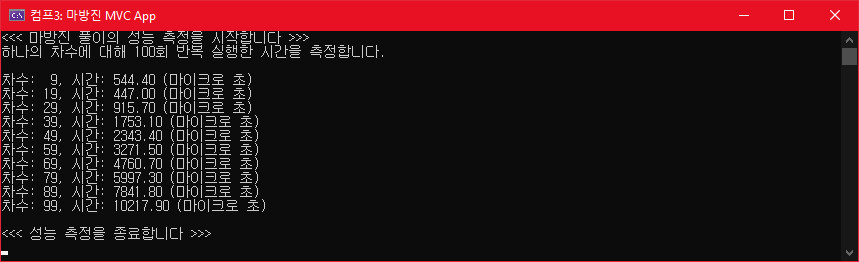
\includegraphics[width=\textwidth]{test_result_wrong_with_debugger.png}
                \caption{여러 요소에 의해 측정값이 잘못 나온 결과}
                \label{}
            \end{figure}    
            
            \paragraph{%\
                \normalfont 성능 측정은 현재 CPU에 로드되어 있는 프로세스의 종류나 양에 따라 영향을 많이 받는다. 기본적으로 성능 측정 프로그램 또한 운영체제에 의해 제어되기 때문에, 동작하는 도중 타 프로세스로 컨텍스트 스위칭이 이루어질 수 있으며 이는 처리 시간의 증가로 이어진다.
            }

            \paragraph{%\
                \normalfont 이는 프로그램의 빌드 과정도 예외가 아니며, 막 빌드가 끝난 이후 바로 프로그램이 실행될 경우 메모리 정리 과정이나 캐시 미스 등의 이유로 성능 측정이 잘못 이루어질 수 있다. 
            }

            \paragraph{%\
                \normalfont 따라서, 두가지 경우의 해결책을 제시할 수 있다. 단, 실행 중인 프로그램을 전부 종료한다는 조건을 상정한다: 
            }
            
            \begin{itemize}
                \item 실행 후 바로 \texttt{AppController}를 호출하지 않고 \texttt{Sleep} 등으로 대기하여 CPU가 idle 상태에 들어갈때까지 기다리기
                \item 빌드된 프로그램을 별도로 실행하기
            \end{itemize}

            \paragraph{%\
                \normalfont 본 보고서에서는 전자의 경우를 선택하여 적용하였으며, 실제로 실행 후 5초간 대기한 후 본 로직을 실행한다. 
            }

    \chapter{실행 결과 분석}
        \begin{figure}[h]
            \centering
            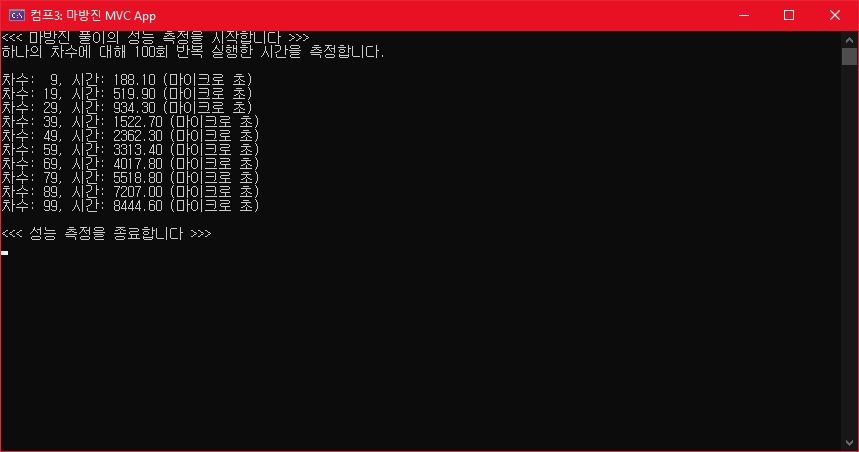
\includegraphics[width=\textwidth]{test_result.png}
            \caption{실행 결과}
            \label{fig:result}
        \end{figure}
        
        \begin{figure}[h]
            \centering
            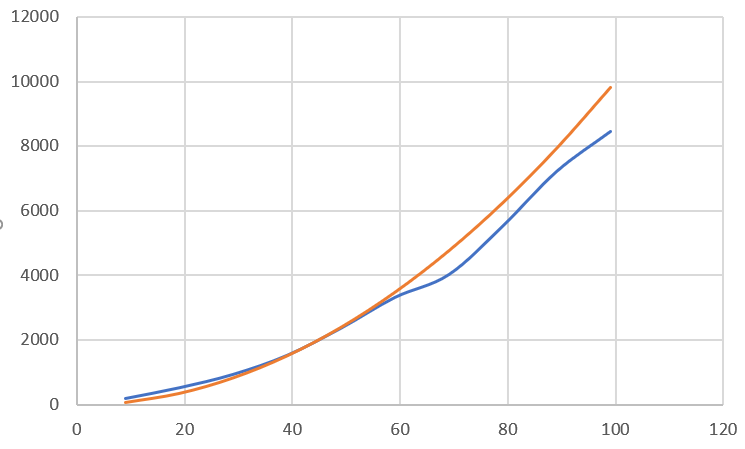
\includegraphics[width=\textwidth]{chart.PNG}
            \caption{$n^2$ 와 비교 (주황색: $y=x^2$, 파란색: 실측값, 단위: 마이크로초)}
            \label{fig:comparison}
        \end{figure}
        
        \section{입력과 출력}
            실습 자료에서 제시된 입력을 사용하였으며 출력 결과는 ~\ref{fig:result} 및 ~\ref{fig:comparison} 와 같았음.
        \section{결과 분석}
            각 구간에서 측정된 실행 시간의 증가가 대체적으로 예측값에서의 증가와 대체적으로 유사함을 확인하였음.

    \chapter{소스코드}
        소스코드는 제출된 압축파일에 같이 동봉되어있으며 GitHub (0x00000FF/CNUCSE-Computer-Programming-III-2020-Spring) 에서도 열람할 수 있다.
\end{document}